% ビルドメモ
% bibtex では、うまくいかない。
% jbibtex はインストールされていない。
% pbibtex を使うと旨くいく。
% 次の手順でうまくいく。
% $ platex template-j
% $ pbibtex template-j
% $ platex template-j
% $ platex template-j
% $ dvipdfmx template-j

%% 和文論文用のテンプレート
%%%%%%%%%%%%%%%%%%%%%%%%%%%%%%%%%%%%%%%%%%%%%%%%%%%%%%%%%%%%%%%%%%%%%%%%%%%%
%% 1. 和文原稿
 \documentclass[originalpaper]{jsaiart}     % 原著論文 Original Paper
% \documentclass[blindreview]{jsaiart}      % 査読用
%
% \documentclass[shortpaper]{jsaiart}       % 速報論文 Short Paper
% \documentclass[exploratorypaper]{jsaiart} % 萌芽論文 Exploratory Research Paper
% \documentclass[Specialissue]{jsaiart}     % 特集 Special Issue
% \documentclass[specialissue]{jsaiart}     % 小特集 Special Issue
% \documentclass[interimreport]{jsaiart}    % 報告 An Interim Report
% \documentclass[surveypaper]{jsaiart}      % 解説 Survey Paper
% \documentclass[aimap]{jsaiart}            % AIマップ AI map
% \documentclass[specialpaper]{jsaiart}     % 特集論文 Special Paper
% \documentclass[invitedpaper]{jsaiart}     % 招待論文 Invited Paper
%

%% ページ番号の指定,掲載時に学会の方で決定します.
% \setcounter{page}{1}
% \setcounter{volpage}{1}


%%% amsmathパッケージの注意点 %%%%%%%%%%%%%%%%%%%%%%%%%%%%%%%%%%%%%%%
% \usepackpage{amsmath}
% 数式番号の参照は \ref ではなく,\eqref を用いること
% documentclass のオプションに fleqnを指定すること
% 例: \documentclass[technicalpaper,fleqn]{jsaiart}

\usepackage[dvipdfmx]{graphicx}
\usepackage{graphics}
\usepackage{fancybox}
\usepackage{comment}

\Vol{12}
\No{1}
%\jtitle{物体検出のためのニューラルネットワークのサーベイ}
\jtitle{物体検出に用いられるニューラルネットワークモデル}
% \jtitle[柱用和文タイトル]{和文タイトル}
\jsubtitle{最新モデルのサーベイと目的に応じたモデルの選択}
%\etitle{A Survey of Deep Neural Networks for Object Detection}
\etitle{Neural Network Models for Object Detection}
\esubtitle{A Survey of the Latest Models and Optimal Model Selections for Specific Tasks}

\manyauthor % 著者が3名以下の場合はこの行を消すこと

%%% 著者名の注意点 %%%%%%%%%%%%%%%%%%%%%%%%%%%%%%%%%%%%%%%%%%%%%%%%%%%
% 所属先が同じ著者が連続する場合,その中の先頭の著者のみ \affiliation
% を用い,残りの所属先には \sameaffiliation を使う
% ただし,所属先が同じでも連続していない場合は \affliation を使う
% 名前が長い場合は \name の代りに \longname を使う

\author{%
 \name{金子}{純也}{Junya Kaneko}
 \affiliation{Morning Project Samurai 株式会社}%
     {Morning Project Samurai Inc.}%
     {junya@mpsamurai.com, http://www.mpsamurai.com}
%\and
% \name{著者2姓}{名}{Auther2 Roman Name}
% \affiliation{日本語所属名2}%
%     {Affiliation2 in English}%
%     {user2@ai-gakkai.or.jp, http://www.ai-gakkai.or.jp/~user2/}
\and
 \name{山田}{貢己}{Miki Yamada}
 \sameaffiliation{m.yamada@mpsamurai.com}
%\and
% \longname{カタガナガキノ}{ナガイナガイナマエ}{VeryLong Roman Name}
% \sameaffiliation{user4@ai-gakkai.or.jp, http://www.ai-gakkai.or.jp/~user4/}
%\and
% \name{著者5姓}{名}{Auther5 Roman Name}
% \affiliation{日本語所属名1}%
%     {Affiliation1 in English}%
%     {user5@ai-gakkai.or.jp, http://www.ai-gakkai.or.jp/~user5/}
}

\begin{keyword}
%キーワードとして,小文字(固有名詞や略語を除く)の英単語を2〜5個指定
    survey, neural network, object detection, instance segmentation, deep learning
\end{keyword}

\begin{summary}
「ショートノート」は 200 ワード,それ以外は200〜500 ワード
以内の英文でsummaryを記す
(ここは,論文執筆後に書く.)
\end{summary}

\begin{document}
\maketitle

★ここにチートシートを出力する.
\section{まえがき}
%■ 本論文の目的:誰(理工系大学2年生)を対象に、何(物体検出の始め方)を伝えるか
%\subsubsection*{この論文の狙い}
{\bf この論文の狙い:\ }このサーベイは,理工系大学2年生程度の数学の知識を前提に,物体検出をこれから始めるにはどうすればよいかという道すじを伝えることを目的として執筆したものである.物体検出でできることは何?から始まり,物体検出をするために必要なもの(ハード,ソフト,データ,知識,明確な目的)を簡潔に纏めてある.また,読者にとっての理想的なサーベイ(即時性,分かりやすさ,一言で説明,参考文献は充実)というものの一つの解として,随時更新されるGitHub上の(日本語で書かれた)物体検出まとめサイトとライブラリを紹介する.

%■ 最近の世の中の状況のおさらい
{\bf 世の中の状況:\ }近年,「AI(人工知能)」という言葉が国内外に蔓延しており,技術者のみならず一般の人の日常生活にもすっかり浸透した.常に手の届くところにAIがあり,AIに囲まれて生活していると言っても過言ではない.テレビやインターネットの画像は,本物と見間違えるほどの人工画像で溢れ,スマホや机上のスピーカーに話しかけるとあらゆる情報を教えてくれるばかりでなく,電化製品を操作することもできるようになった.高速道路を自動運転する車も増えている.

%■ AI分野(画像認識分野)における物体検出の位置づけ
{\bf AI分野における物体検出:\ }ここ数年で飛躍的に性能を向上させたAI関連技術は,画像認識,物体検出,ロボット制御,音声認識,機械翻訳,ビッグデータ分析などであり,これらの多くの領域で深層ニューラルネットワーク(Deep Neural Network(DNN))が使われている.とりわけ画像認識分野でこのDNNが注目されるようになったのは,2012年に開催された最先端の一般物体認識の性能を競うコンテスト ILSVRC においてDNNを使った手法が他の手法に大差をつけて優勝したことが発端である.「画像中の物は何か?」に答える物体認識をさらに進めて,「画像中のどこに何があるか?」に答えようとするものが本論文のテーマ「物体検出」であり,現在のAIブームを巻き起こした源流がここにあると言ってよい.

%■ 物体検出でできること
{\bf 物体検出でできること:\ }物体検出とは,カメラで撮影された画像データを電子的に処理し,予め登録しておいた物体(例えば,人,犬,猫,自動車,飛行機,...)を見つけ出し,その正確な画像上の位置と物体の種類を予測するものである(「予測(predict)」は,「推定(estimate)」,「推論(inference)」などとも呼ばれ全て同じ意味で使われる).

現在の標準的方法においては,予め,検出したい対象の学習データ(物体が写っている画像,物体の種類,物体の位置を示す矩形の座標)を大量に用意し,画像を入力すれば種類と位置を出力するように,ニューラルネットワーク等の予測モデルを学習させる.通常,これに数時間から数日要すると言われている.

学習が完了した予測モデルの能力は,タスクの種類によっては人間の能力(予測結果のスコアの平均値)を超えたと言われているものもある(物体認識など).ただし,物体が写し出された画像の品質(解像度,ノイズ,露出不足/過多)や撮影アングル(遮蔽物,変形,大き(小さ)過ぎる)に問題がある場合は性能が低下することは避けられない.

物体検出と似た技術として,次の3つがある:

\begin{itemize}
    \item セマンティックセグメンテーション(全画素の物体の種類を認識するが,同種の物体同士は区別しない)
    \item インスタンスセグメンテーション(同種の異なる個体を区別して物体検出を行い,且つ,画素単位で個体の識別をする)
    \item パノプティックセグメンテーション(全画素の物体の種類を認識し,同種の異なる個体も区別する)
\end{itemize}
本論文では上記のセグメンテーション技術も含めた広い意味での物体検出について述べる.

%■ 物体検出をするために必要なもの(ハード、ソフト、データ、知識、明確な目的)
{\bf 物体検出をするために必要なもの:}

\begin{description}
    \item[ソフトウェア] 
    \begin{itemize}
        \item PyTorch/TensorFlow 等の深層学習ライブラリとその稼働環境(Linux/Windows/Mac上のPython, jupyter notebook環境など).
        \item 物体検出を行うソフトウェア(予測モデルの作者,または,物体検出を行おうとする担当者が作ったもの).
    \end{itemize}
    \item[ハードウェア] 
    \begin{itemize}
        \item 前記ソフトウェアが実行できる環境(PC(GPUがあると良い), 或いは,Google Corabolatory などのサーバ上の実行環境).
    \end{itemize}
    \item[データ] 
    \begin{itemize}
        \item 学習データ(事前学習用,並びに,fine-tuning用の入力と出力のペア)
        \item 本来処理したいデータ(入力).
    \end{itemize}
    これらは,使用するソフトウェアで読み取ることのできる状態にしておく(データの前処理).
    \item[知識] 物体検出のソフトウェアを使うには,入出力データの意味を理解する必要がある.特に,予測モデルの出力データは通常は誤差を含むものとなるため,出力が表す数値が確率値を表すのか,何らかの物理量を表すのか,分類のカテゴリを表すのか,正確に把握する必要がある.また,学習時の損失関数の値から,予測モデルの推定誤差を見積もることができるのだが,それには出力結果を正しく解釈できる統計学の知識が必要となる.
    \item[明確な目的] 何がしたいのかということを明確化しておくことがが,物体検出を行おうとするときに重要となる.物体検出は新しい技術であり,標準的な統計解析の手法よりも手間と計算コストが大きくなりがちである.他の方法では解決できないのか?と問いかけて,本当にこれが必要であることを確認しておくべきである.
\end{description}

%■ 良いサーベイとは(即時性、分かりやすさ、一言で説明+参考文献)(随時更新する)まとめサイトとライブラリ(GitHub)の紹介。
{\bf 理想的なサーベイとは:\ }最新技術のサーベイ論文は,有用であり様々な分野で昔から(論文雑誌が生まれた頃から)活用されていると思われる.しかしながら,進歩の速い分野においてはサーベイが出た頃には既に内容が古くなってしまっているという問題が往々にして起こる.また,とても良く書かれたサーベイほど内容が濃く多くなり,執筆に時間と労力を要するのはもちろん,それを読み解くのにも時間を要するということもよくある.

我々は,github上に随時更新される形式でサーベイを公開することを試みた.出版されたときには既に古くなっているという懸念を取り払える可能性を期待している.また,この分野に新規参入しようとしている人がなるべく短時間で必要な情報にたどり着き,取り組んでいる問題を解決する最適な方法を見つけたり,或いは,新たな研究に取り組めることを目指し,内容の拡充性や緻密性よりも,なるべく視覚的に解りやすいコンパクトな内容になるよう心掛けた.

\section{物体検出(Object detection)}
%\begin{figure}[t]
%    \begin{center}
%        \includegraphics[width=8cm,clip]{fig/test_fig2.eps}
%    \end{center}
%    \caption{ 図の説明文 ... }
%\end{figure}
\subsection{物体検出器(object detector)の働き}
{\bf 基本動作:\ }物体検出器は,画像(1枚の静止画をファイルにしたもの)を処理し,処理結果(検出個数,検出物体の画像座標,検出物体の種類)を出力する.セグメンテーションの場合は,出力解像度(画像のサイズ)に応じた各画素のクラス分類結果も出力される.画像を読み込ませる際には,幅と高さを含む情報も与える必要がある.検出器によっては画像サイズや画像ファイル形式が指定されているものもあるのでその場合は,予め画像ファイルを変換する前処理が必要となる.

{\bf 出力結果の見かた:\ }検出座標は物体を囲む矩形(bounding box (以下,bbox))の座標を4つの数値で表すことが多い.また,検出の信頼度が0.0〜1.0の実数で出力される場合はそれが推定正答確率を表すように設定されている.

{\bf 学習のしかた:\ }学習データは,推論実行に必要なデータに正解データを加えたものであり,いわゆる教師あり学習を行わせる.ただ,推論時には無い学習に関するパラメタの設定をしなければならない.検出器の構成(中間層の層数,特徴量次元のサイズ,検出器独自のパラメタなど)もこの段階で設定する.通常は,確率的降下法でモデルのパラメタを学習させることが多く,検出器の重みパラメタの初期化方法(平均,分散,値を指定など),最適化方法(SGD, Adam, 他),学習率のスケジューリング,学習打ち切り基準,ミニバッチサイズなどを指定する.学習時には交差検証を行わせて未学習データに対する誤差も計算させることができるので,その誤差を控えておくことにより推論時の予測精度を見積もることができる.

{\bf 事前学習(pre-training)と事後学習(post-training, fine-tuning):\ }世界最高性能を出すほどの検出器の学習は,たいてい事前学習と事後学習の2段階で行われる.事前学習は主に公開データベースなどの大量データを用いて検出器の前半部分を学習させて適切な内部表現を獲得するために行われる.検出器によっては事前学習済みの重み係数パラメタが公開されているものもある.事後学習は,最終目的に合致したデータを追加して,場合によっては検出器の最終層を追加して,所望の検出処理を実行できるように最終調整の意味合いで実施するものである.事前/事後学習のやり方は各検出器によって異なるため,説明書きや論文等に記された方法を参考にして実行する必要がある.

%{\bf Two-stage 検出器と one-stage 検出器:\ }
物体検出器は次の2種類に分類できる\cite{JZLYLFQ19}:
\begin{description}
    \item[Two-stage 検出器] 高い位置決め精度と物体認識精度をもつ(Faster R-CNN など).最初のCNNベースの物体検出器 R-CNN とその改良手法はこの方式である.次の2つのstageで処理される:
    %\begin{description}
    \begin{itemize}
        \item 第1 stage: 物体の bbox の候補を選出する.Faster R-CNN では Region Proposal Network (RPN) と呼ばれている.
        \item 第2 stage: RoI Pooling が各候補boxから特徴量を切り出し,後続の分類器と bbox 回帰器がそれを処理する.
    %\end{description}
    \end{itemize}
    \item[One-stage 検出器] 推論速度が高速である(YOLO, SSD など).Region proposal をせずに直接,入力画像から bbox を検出して出力する.近年では,改良により検出精度も向上している.
\end{description}

\subsection{Two-stage検出器}
\subsubsection{Faster R-CNN}
代表的なtwo-stage検出器であり,物体検出に対して当時の最高性能を達成しながら,処理速度の点でも大きく改善したモデルである\cite{RHGS15}.
PASCAL VOC 2007 に対して mAP=69.9\% の精度を 5fps で達成した.
\begin{figure}[tb]
    \begin{center}
        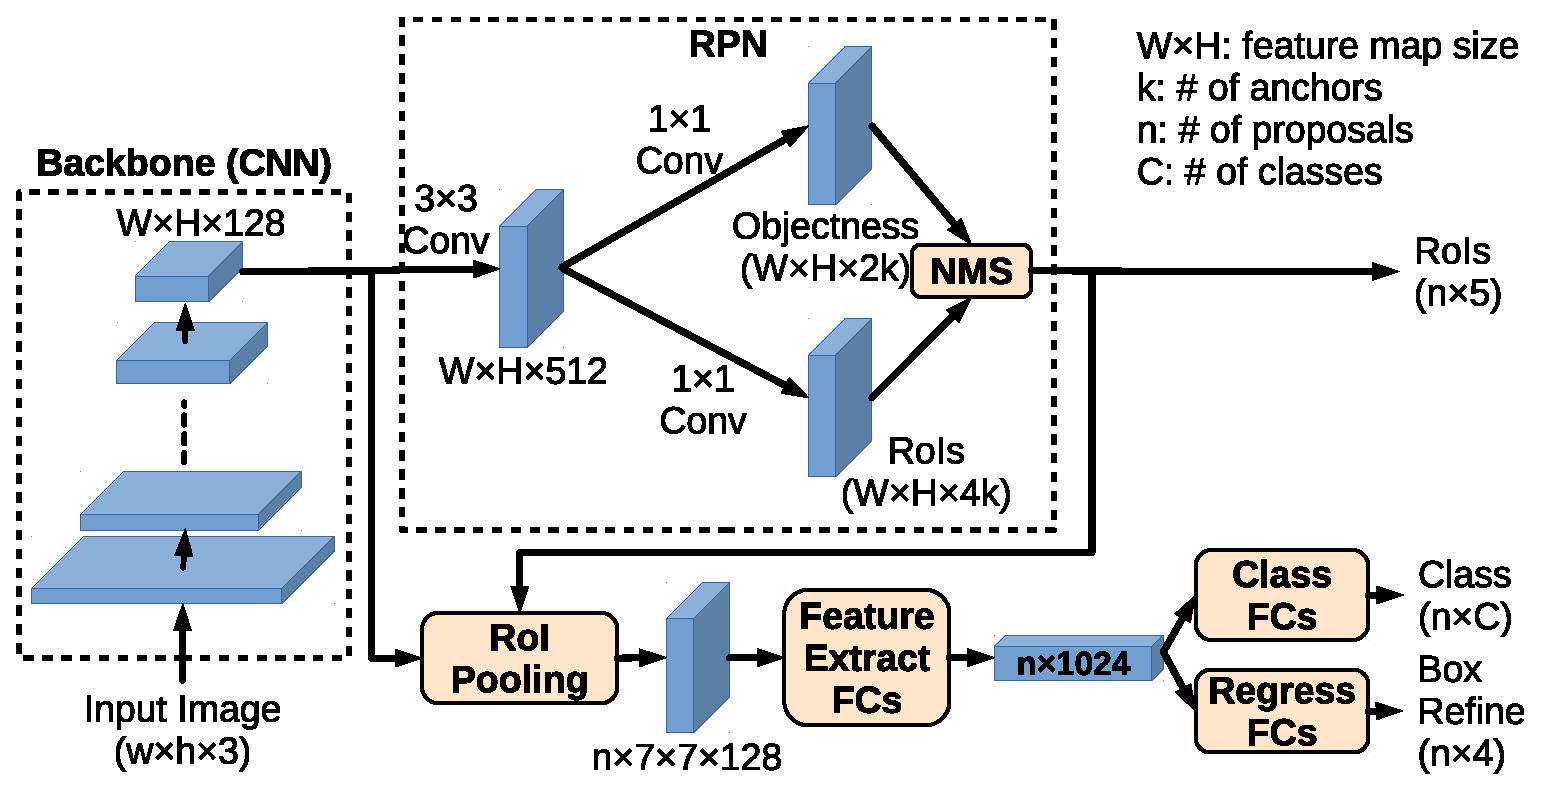
\includegraphics[width=8cm,clip]{fig/archi_FasterRCNN.eps}
    \end{center}
    %\capwidth=90mm %
    \caption{ Faster R-CNN の構造.}
    \label{fig:archi_FasterRCNN}
\end{figure}

{\bf Faster R-CNN の構造:\ } \ref{fig:archi_FasterRCNN}に示すように,backbone,Region Proposal Network (RPN),RoI Pooling,特徴抽出ネットワーク,分類器,回帰器で構成される.

Backbone は CNN で構成され,$W{\times}H{\times}128$のサイズの特徴量を出力する.提案当時はVGG-16 \cite{SimZis15}などが用いられた.

RPN は backbone が出力した特徴量をさらに CNN で処理して物体の種類に依存せずに物体を検出してその候補(proposalと呼ぶ)の RoI (bbox座標)と物体らしさ(objectness)を $n$ 個ずつ出力する.RPN内部では特徴量をCNNで変換し,特徴量の各空間座標点毎に $k$ 個の「bbox(4個) と物体らしさ(2個)の数値」を同時に出力している(計$WH(4{+}2)k$個).これらの bbox は non-maximum suppression (NMS) によって,物体らしさが閾値を超えているものだけを残し,また,1個の物体を複数回検出したものも1個だけに集約することにより,RPNが出力するproposal を $n$ 個以下に抑える.ここで,各座標点に割り当てられた $k$ 個の初期 bbox を anchor box と呼んでいる.

RoI Pooling は,backbone からの特徴量と RPN からの $n$個の proposals を受け取り,bbox内部の特徴量を切り出して物体の大きさにかかわらずに空間サイズを 7{$\times$}7 の固定サイズに変換する.

固定サイズの特徴量は,共通の特徴抽出を行う全結合(Full Connect)層(以下,FC層)により $n{\times}1024$のデータに変換され,分類器と回帰器に送られて別々のFC層で処理されて,クラス分類確率と bbox 調整量がそれぞれ出力される.(★bbox調整量が全クラス分出力されるのかどうか確認要!)

{\bf Faster R-CNN の学習:\ } 
\begin{enumerate}
    \item CNNによる特徴量生成は,画像認識などの学習で構築された重みを初期値として fine tuning を行う.
    \item RPNだけをEnd-to-Endで学習.anchorと教師データに基づき,物体か背景か(物体らしさ,2k個)と,anchorからのずれ(4k個)を学習.
    \item RPN固定で全体を学習する.RPNのRoI出力を全体の出力及びRoI poolingへ送り,特徴抽出器で分類と回帰の共通部分のFC計算を行う.分類器はクロスエントロピー,softmax などで計算し,回帰器が行う線形回帰はL1ノルムで学習し,bboxの位置の補正を行う.
\end{enumerate}

\subsubsection{Two-Stage Fine-Tuning Approach (TFA)}
Few-shot 物体検出のためのシンプルな Two-stage によるfine-tuning法である\cite{WHGDY20}.
元来,深層学習は膨大な個数の学習データが必要であり,実用上の観点では学習データを集めることが困難な事象の一つであった.それゆえ,少ないサンプルから珍しいオブジェクトを見つけることを目的とする few-shot 物体検出の開発が進められている。
few-shot 学習の方法としてはメタ学習が有望と見られてきたが,このTFAはそれまで注目されてこなかった fine-tuning に焦点をあてることで大きな性能向上をもたらした.
最終層のみ fine-tuning することが few-shot 物体検出にとって重要であることを発見し,それを用いた Two-stage Fine-tuning Approach (TFA)を提案した.
メタ学習の従来手法よりも 2〜20ポイント優れた性能を出している.ただし,少数サンプルの分散が大きいと信頼性が低下することに注意が必要である.
モデルの構造は,Faster R-CNNがそのまま使われている.本手法は,ネットワーク構造には殆ど依存しない.few-shot学習方法に特徴がある.

\begin{figure}[tb]
    \begin{center}
        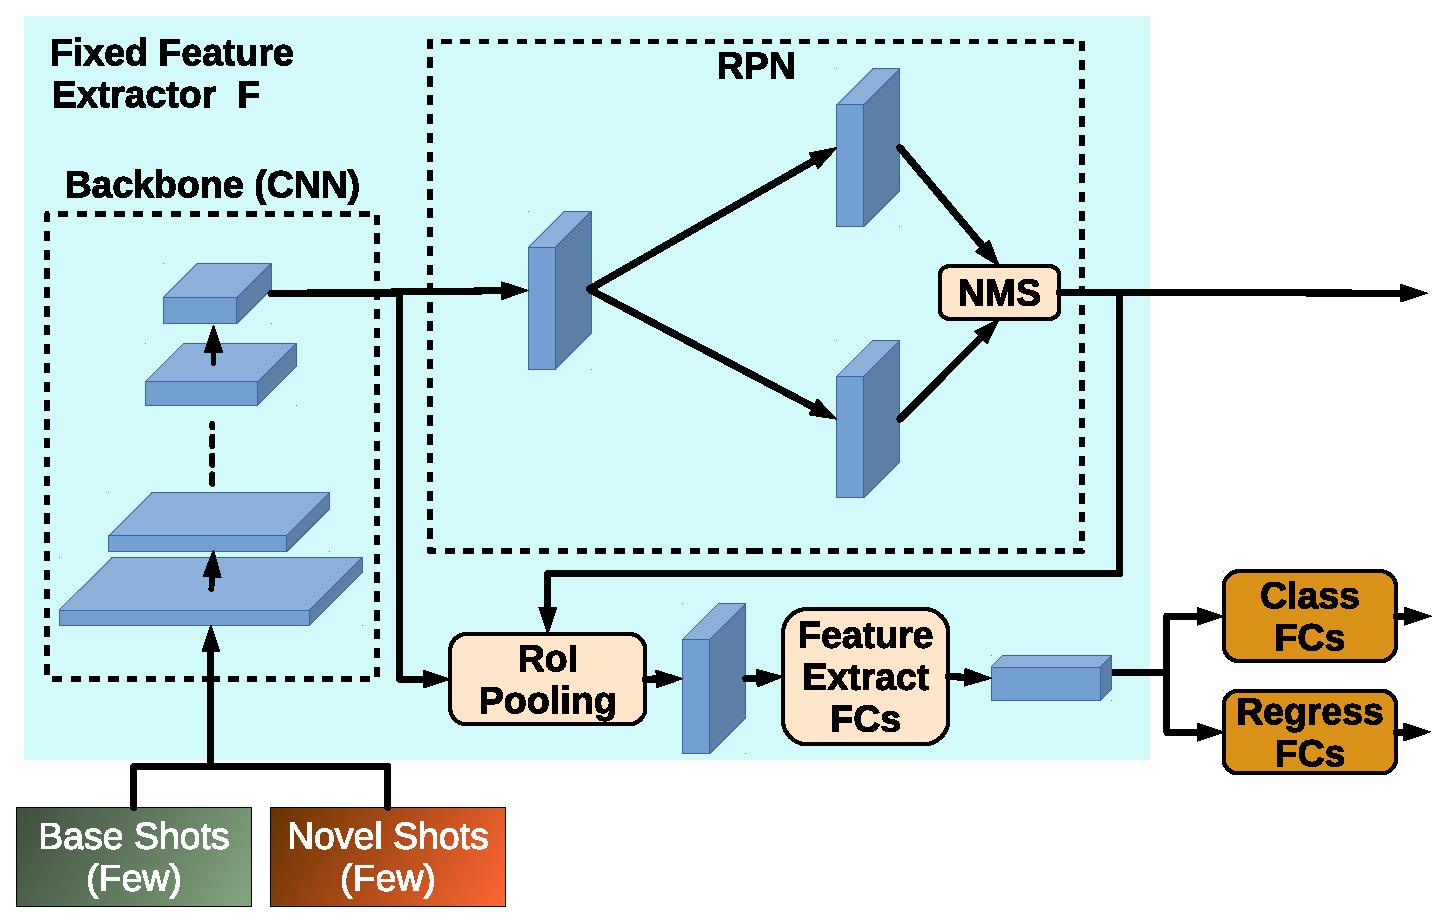
\includegraphics[width=8cm,clip]{fig/archi_TFA.eps}
    \end{center}
    %\capwidth=90mm %
    \caption{ Stage 2: Few-shot fine-tuning.}
    \label{fig:archi_TFA}
\end{figure}
{\bf Two-stage fine-tuning approach (TFA) の学習:\ } 
\begin{enumerate}
    \item aabb
\end{enumerate}

\subsubsection{Few-Shot Object Detection}

\subsection{One-stage検出器}
\subsubsection{YOLOv4}
\begin{figure}[tb]
    \begin{center}
        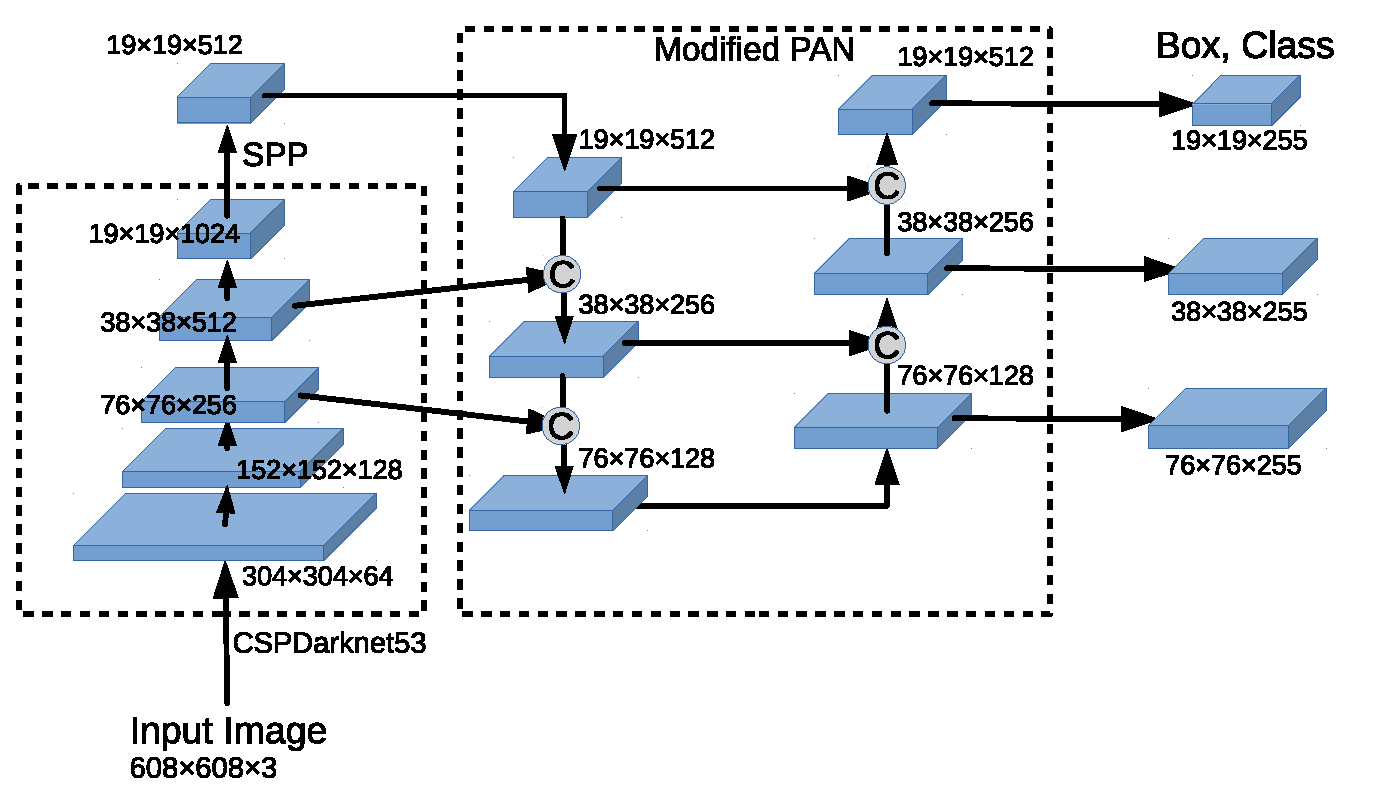
\includegraphics[width=8cm,clip]{fig/archi_YOLOv4.eps}
        %\includegraphics[width=8cm,clip]{fig/testYOLO.eps}
    \end{center}
    %\capwidth=90mm %
    \caption{ YOLOv4 の構造.}
    \label{fig:archi_YOLOv4}
\end{figure}
代表的なone-stage検出器であり,高速,高性能で軽量であることが特長である\cite{BWL20}.YOLOv3までの特徴を継承しつつ,採用可能なbackbone,neck, head から最適な組み合わせを選択し,また,適用可能な各種技術を取り込んで構成された(\ref{fig:archi_YOLOv4}).

{\bf YOLOv4の構造:\ }入力画像は,backbone(画像の特徴を抽出する処理(縦横サイズを小さくしながら特徴量を含むチャネルを増やしていくこと)),neck(FPNやPANのように、特徴量ピラミッドを昇り降り横断する処理),head(「backbone + neck」が出力する特徴量から、クラス信頼度とbounding boxオフセットを推論するネットワーク)の順に処理される.

backbone である CSPDarknet53 は,YOLOv3 で使われた Darknet53 に Cross Stage Partial Network (CSP)を導入したものである.Darknet53 は,residual結合を持ちConvolution 2層で構成されるブロックが多数積み重なった構造であり,名前の53はConvolutionが53個あることから来ているとしている(ただし,53番目の層は全結合層である).CSP network は予測性能を向上させる工夫であり,注目するブロックへの特徴量入力を2つに分割し,一方はそのブロックで処理し,もう一方は処理をスキップしてそのまま送り,これら2つを連結(concatenation)して出力することを行う.ただし,YOLOv4においては,この「分割」処理の代わりに,分岐させた直後にstride=2のConvolutionで処理して両方のチャネルサイズを1/2にしている.

CSPDarknet53のTopの出力はSPPモジュール(kernel size={1, 5, 9, 13}, stride=1として,4つ並列にmax poolingを行い,これらをconcatするもの)に送られる.比較的大きなk$\times$k max-poolingが効果的にbackbone特徴量の受容野を増加させてから,neckのTopに渡される.

neck である Modified PAN は,Path Aggregation Network (PAN)(3つのピラミッドを行き来して高解像度情報を特徴マップに効果的に伝えるモデル)におけるbottom-up path の加算計算をconcatenationに変更したモデルが用いられている.

ここではさらに,Modified Spatial Attention Module (SAM)(Convolutionの出力を2つに分岐し,一方にConvolution + sigmoid処理を行い,元信号に掛け算する)の演算を行ったものがPANの3個の出力としてheadに渡される.

3つのheadは,それぞれ独立にconvolution計算を2回行い,最終的なクラス信頼度とbounding boxオフセットを出力する.

{\bf YOLOv4の学習:\ }一般的な確率的降下法を用いた学習に加えて,いくつか効果的な学習の工夫を導入している: 

\begin{description}
    \item[CutMix] 学習画像の一部を切り取ったパッチを別の学習画像の一部に貼り付けて,正解ラベルもパッチの面積に比例させてミックスしたものを生成してそれで学習する.
    \item[Mosaicデータ拡張] CutMixを,4つの画像を用いるように拡張したもの.
    \item[DropBlock] 特徴マップに対して,無作為に選出した矩形範囲(block)にマスクを掛けたもので学習する.
    \item[Class label smoothing] クロスエントロピー損失で学習する際に,logitが発散しないように正解ラベルを$q'(k|x)=(1-\epsilon)\delta_{k,y}+\epsilon/K$とした損失を用いて学習する.
    \item[Complete IoU (CIoU) 損失] 二つのbounding boxが離れていても,近づきすぎていても適切な損失関数になるように,IoU損失を改良した損失関数.
    \item[CmBN] batch normalizationを(ミニバッチ複数回につき1回の重み更新を行う場合に)ミニバッチをまたいで「平均,分散」を蓄積して,重みの更新のタイミングで,biasとscaleを更新するようにしたものである.
    \item[Self-adversarial-training (SAT)] まず,物体を写した元画像を改変し,物体が存在しない画像であると騙す画像を生成する.次に,この改変された画像中の物体を検出するように通常の学習を行う.
    \item[Cosine annealing scheduler] コサイン関数の半周期の形状を利用して,学習率を少しずつ減少させる.これを周期を増やしながら複数回繰り返す.
\end{description}
\subsubsection{EfficientDet}
\section{インスタンスセグメンテーション(Instance segmentation)}
\subsection{Mask Scoring R-CNN (MS R-CNN)}
%\begin{figure*}[b] %これにすると独立したページに1段組で出力された.
\begin{figure}[tb]
    \begin{center}
        \includegraphics[width=8cm,clip]{fig/archi_ms_rcnn.eps}
    \end{center}
    %\capwidth=90mm %
    \caption{ Mask Scoring R-CNN の構造.}
    \label{fig:archi_ms_rcnn}
\end{figure}
マスク品質(インスタンスマスクと正解マスクとのIoUとして定量化されるもの)を分類スコアと明示的に関連付けたモデルである\cite{HHGHW19}.MS R-CNN は,予測マスクの品質を学習するためのブロック(MaskIoU Head)を,Mask R-CNN\cite{HGDG17} に導入したモデルになっている(\ref{fig:archi_ms_rcnn}).MaskIoU Headはインスタンスの特徴量と対応する予測マスクを一緒に取り込み,それを元にMask IoU を回帰推定する.そして,推論時に予測MaskIoUを分類スコアに掛け算して補正する.
\subsubsection{MS R-CNN の学習}
学習サンプルとして RPN proposals を使う.
proposal box と正解box との IoU が 0.5 以上の学習サンプルが必要となる.これは Mask R-CNN の Mask head の学習サンプルの場合と同じである.
各学習サンプルに対する回帰目標を生成するために,まず目標クラスの予測マスクを取得し,予測マスクを閾値=0.5で2値化する.そして,2値化マスクと正解との MaskIoU を使う.
MaskIoUを回帰するのには L2 損失を使い,損失重みは1にする.
ネットワーク全体は end-to-end で学習する.
\subsubsection{MS R-CNN の推論処理}
MaskIoU Head は分類スコア(R-CNN head の出力)の調整に使う.推論の手順は次のようになる:
\begin{enumerate}
    \item R-CNN head が $N$個のbounding boxを出力する.
    \item $N$個のbounding boxのうち,SoftNMS\cite{BSCD17}で上位$k$個のボックスを選択する.
    \item 上位$k$個のボックスを Mask Head に入力し,$k$個のマルチクラスマスクを生成する(ここまでは標準的 Mask R-CNN の手順).
    \item これら$k$個のマスクを目標として MaskIoU Head に入力し,予測 MaskIoU を出力する.
    \item 予測 MaskIoU を,分類スコアに掛け算し,上位$k$個の修正された分類スコアを得る.
\end{enumerate}

\subsection{YOLACT++}
%\begin{figure*}[b] %これにすると独立したページに1段組で出力された.
\begin{figure}[tb]
    \begin{center}
        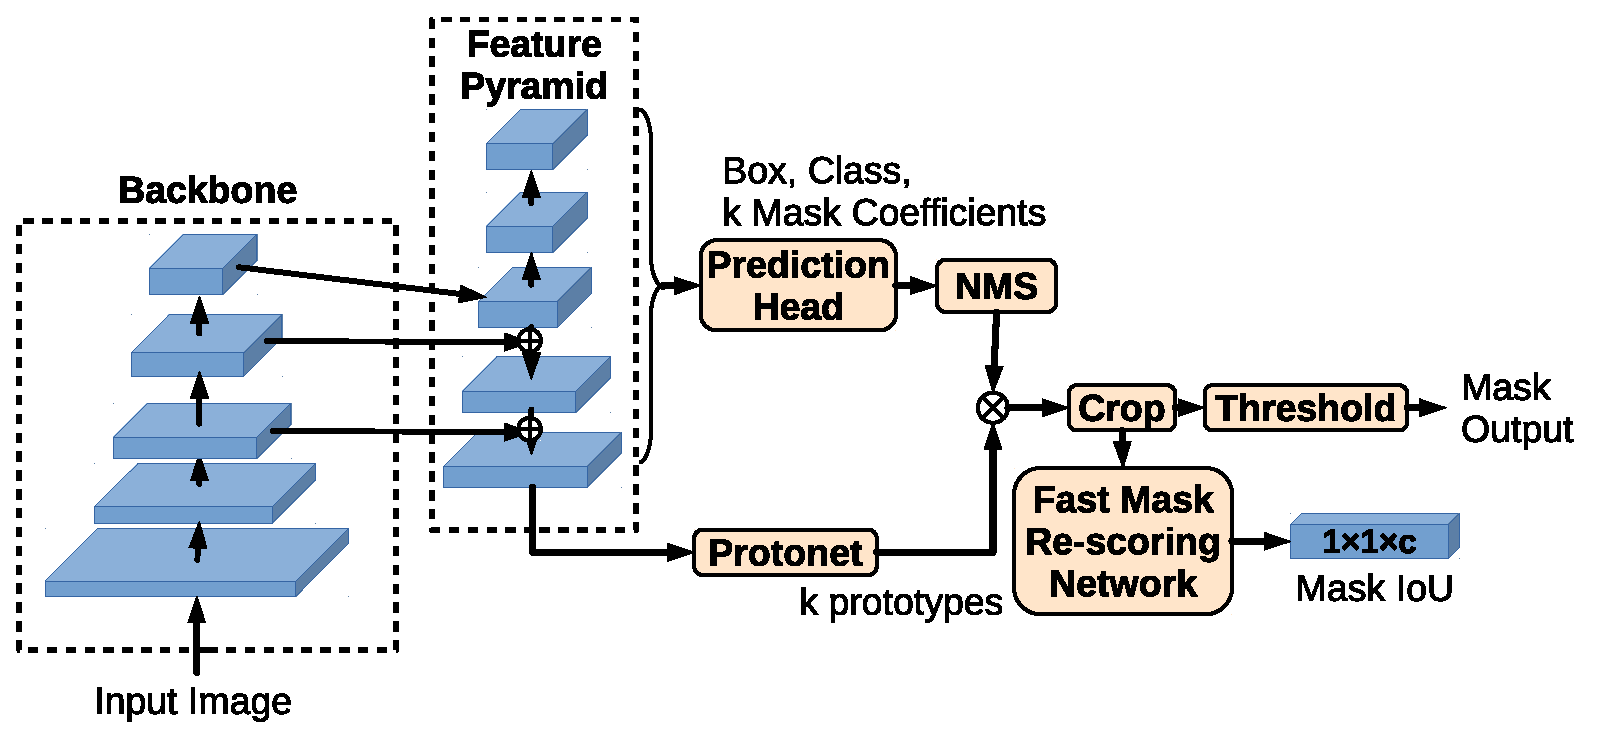
\includegraphics[width=8cm,clip]{fig/archi_YOLACT++.eps}
    \end{center}
    %\capwidth=90mm %
    \caption{ YOLACT++ の構造.}
    \label{fig:archi_yolactpp}
\end{figure}  
実時間(${>}$30fps)で動作するインスタンスセグメンテーションのモデルであり,MS COCO に対して当時の最高性能に匹敵する性能(34.1 mAP at 33.5fps)を達成した\cite{BZXL20}.fully-convolutionモデルであり,deformable convolution をYOLACT\cite{BZXL19}のbackboneに導入する等の改良をしている。物体検出モデルのRetinaNet\cite{LGGHD17} をもとに,インスタンスセグメンテーション向けに改良したものである(\ref{fig:archi_yolactpp}).
\subsubsection{YOLACT++ の学習}
easy negative が多くて学習が困難になる問題は,OHEM法\footnote{入力画像に対する全RoIをミニバッチと考えて、損失の値でソートして識別が難しい negative を選択して学習させる方法.}を用いて negative:positive=3:1 にして学習することで対応する.
Class 信頼度は分類損失(クロスエントロピー),bbox はL1損失,mask (「mask係数×Prototype」で得られるもの)は pixel-wise binary cross entropy でそれぞれ学習する.Re-Scoring Net は Mask IoU(係数)を回帰する学習を行う.

Semantic Segmentation Loss は,学習時のみ接続されるネットワークの学習であり,この学習の実施によりmAPが0.4ポイント向上する.P3特徴量出力に 1×1 convolution 1層で処理してcチャネルの出力をさせて最後にシグモイド関数をかける.これが正解 mask になるように学習する.

%これにより,各画素にc個の[0,1]出力が割り当てられる.
% (おそらく,pixel-wise binary cross entropy 損失と予想)
\subsubsection{YOLACT++ の推論処理}
Prediction Head が各 anchor の Class 信頼度,bbox,k 個の mask 係数を出力し,
Protonet が k 個の Prototype (mask) を出力する.
そして,Predition Head 出力を NMS 処理して選ばれた結果に対して,mask 係数と Prototype を積和した結果(全画面のmask)を,予測 bbox の外側を0で埋めたものを2値化して最終的な予測 mask 出力を得る.

並行して,2値化する前の mask を Re-Scoring Net に入力して,mask IoU 出力を得る.分類スコアは,この mask IoU を掛けて補正される.
\section{パノプティックセグメンテーション(Panoptic(?) segmentation)}
\section{むすび}

\begin{acknowledgment}
謝辞について
\end{acknowledgment}a

%\bibliography{btxsample}
\bibliography{mps}
\bibliographystyle{jsai}

\appendix

\section{付録のタイトル1}
付録の本文1
%\section{付録のタイトル2}
%付録の本文2

% 著者の姓と名の間は半角スペースで区切る
% 略歴は200字以内
\begin{biography}
    %\profile*{m}{著者姓 名}{前掲\kern-.5zw (Vol.X,No.Y,p.Z)\kern-.5zw 参照.}
\profile{m}{金子 純也}{著者1の略歴}
\profile{m}{山田 貢己}{1989年東京大学大学院物理学専攻修了.理学博士.同年株式会社東芝入社.ニューラルネットワークの研究開発,セキュリティ技術,画像認識技術,テレビの高画質化技術,車載画像認識プロセッサ等の開発業務に従事.2020年ジャパニアス株式会社に入社.現在,Morning Project Samurai 株式会社においてAI開発業務に従事.}
\end{biography}

\end{document}
